\section*{Additional Figures}

\begin{figure}[t]
  \centering
  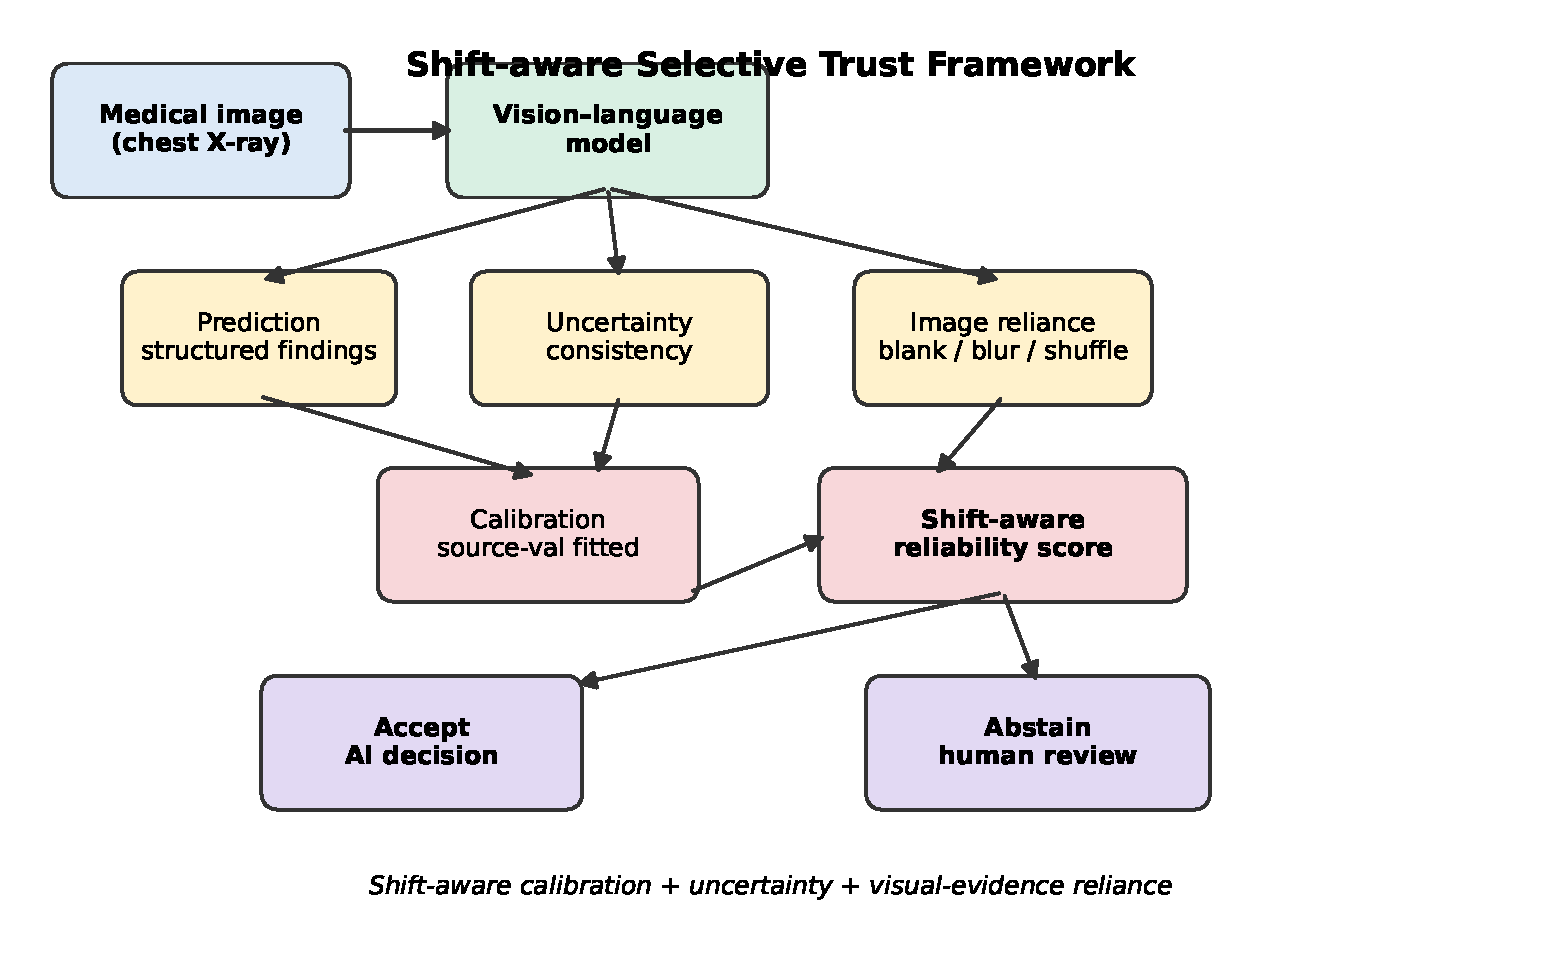
\includegraphics[width=\linewidth]{figures/fig01_framework.pdf}
  \caption{Shift-aware selective trust framework. A CXR VLM produces structured predictions, which are combined with uncertainty, calibration, shift score, and image-reliance evidence to decide whether to accept, clarify, or abstain.}
  \label{fig:framework}
\end{figure}

\begin{figure}[t]
  \centering
  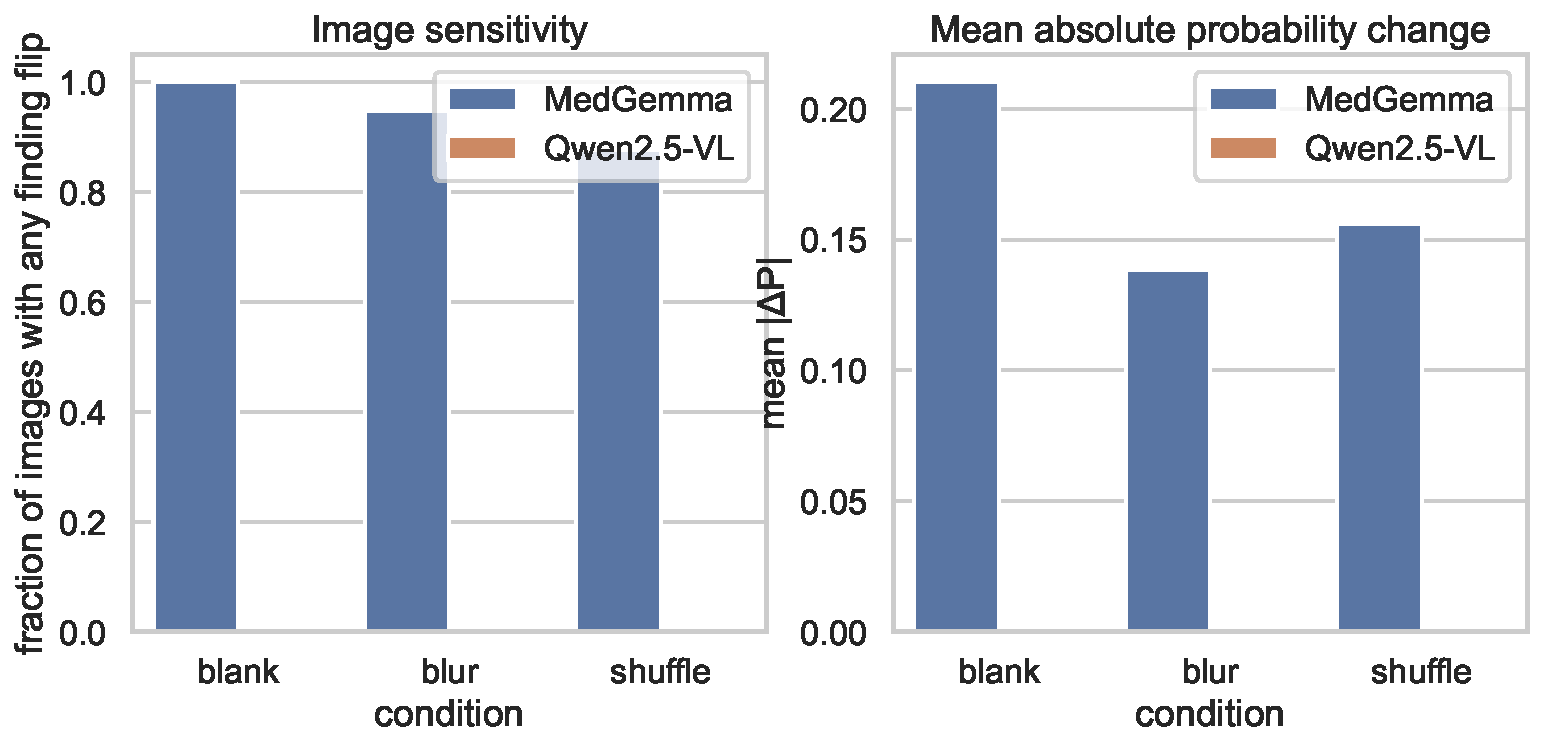
\includegraphics[width=\linewidth]{figures/fig02_image_reliance_main.pdf}
  \caption{Image reliance on 300 NIH studies. MedGemma changes predictions under blank, blurred, and shuffled images, whereas Qwen2.5-VL is effectively image-invariant.}
  \label{fig:image-reliance}
\end{figure}

\begin{figure}[t]
  \centering
  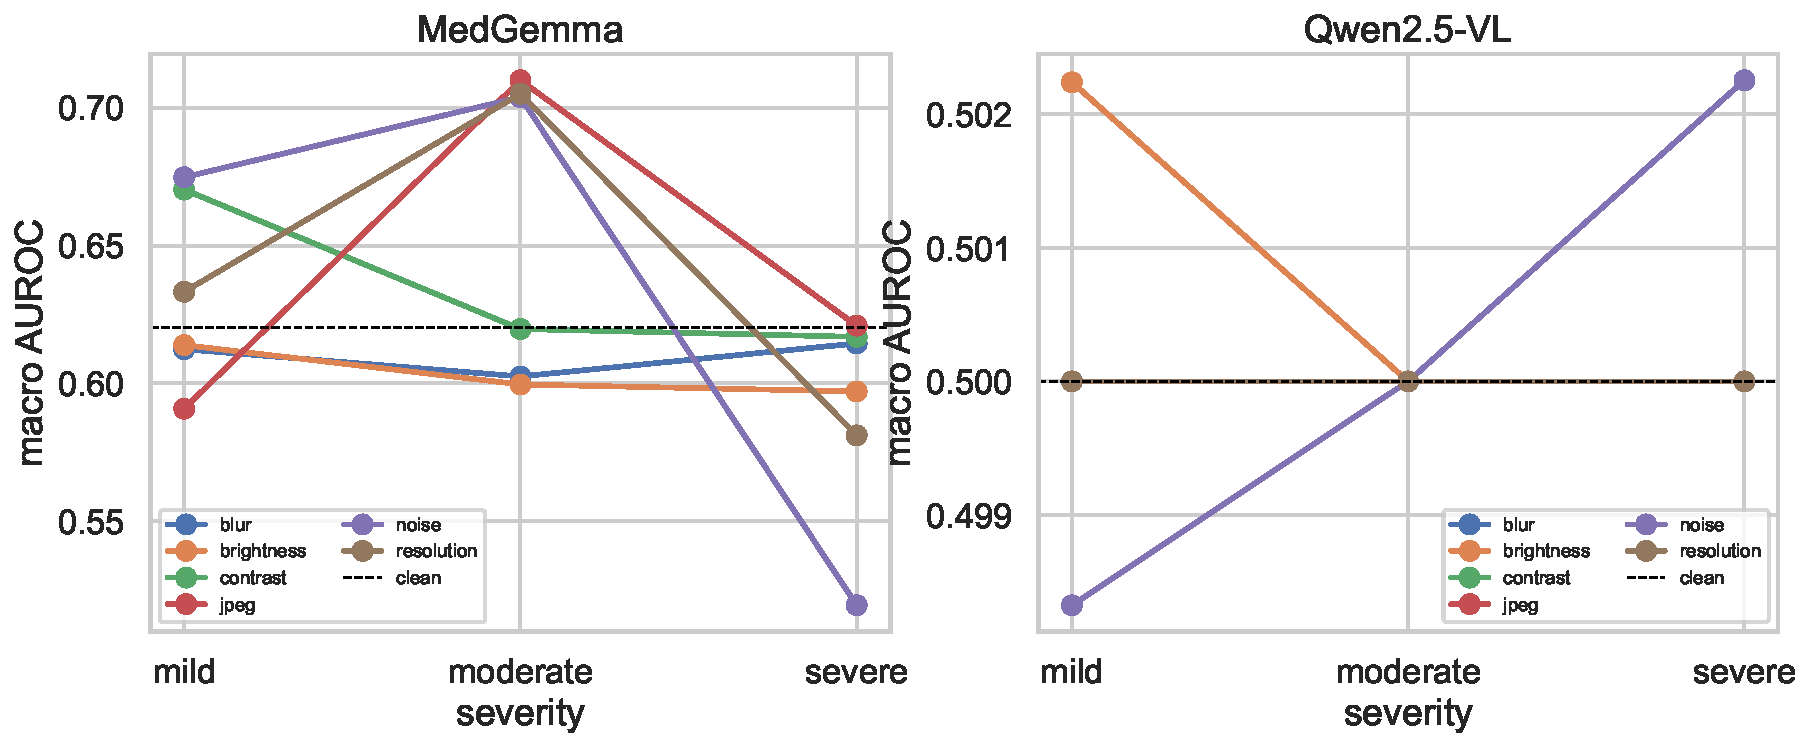
\includegraphics[width=0.49\linewidth]{figures/fig03_shift_auroc_severity.pdf}
  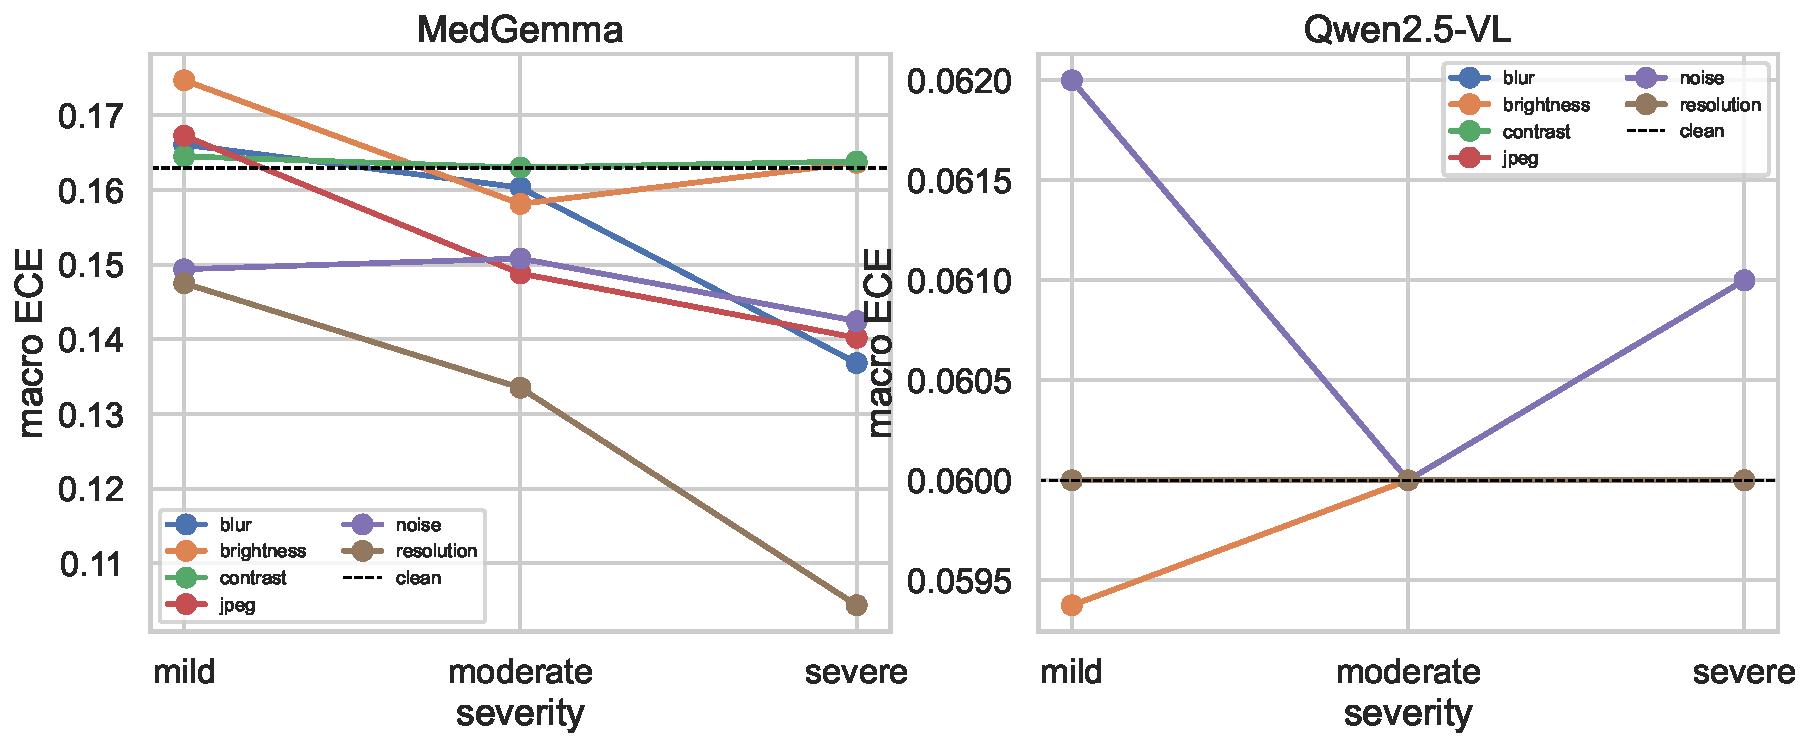
\includegraphics[width=0.49\linewidth]{figures/fig04_shift_ece_severity.pdf}
  \caption{Macro AUROC and ECE under image-quality shift. Shift effects are heterogeneous and non-monotonic; several conditions do not degrade, and sometimes improve, macro calibration.}
  \label{fig:shift-metrics}
\end{figure}

\begin{figure}[t]
  \centering
  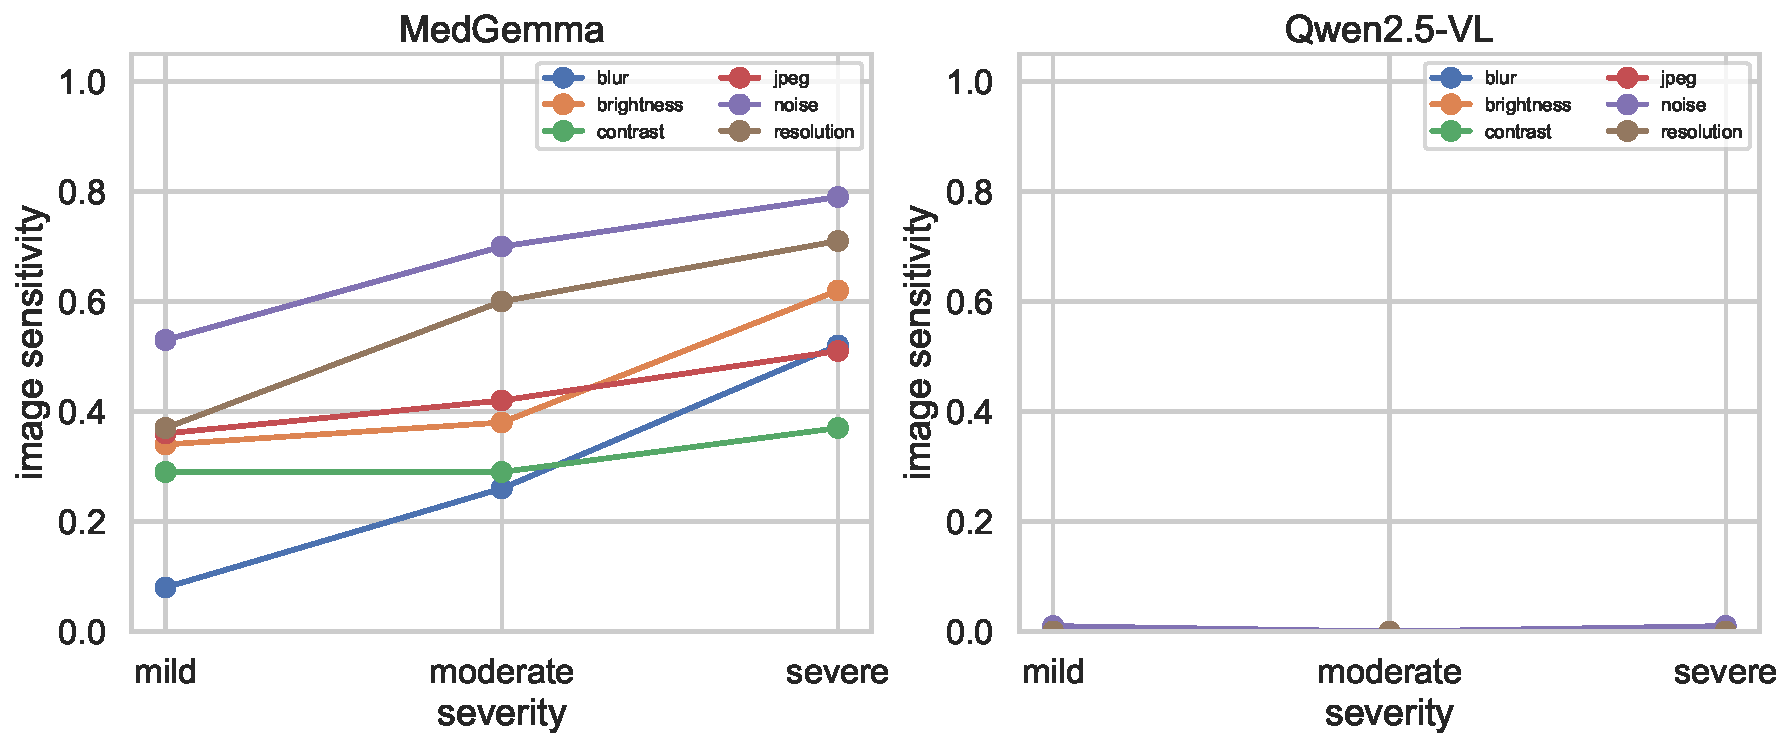
\includegraphics[width=\linewidth]{figures/fig05_shift_image_sensitivity.pdf}
  \caption{Image sensitivity as a function of shift severity. Increasing severity generally increases the fraction of images whose predictions change.}
  \label{fig:shift-sensitivity}
\end{figure}

\begin{figure}[t]
  \centering
  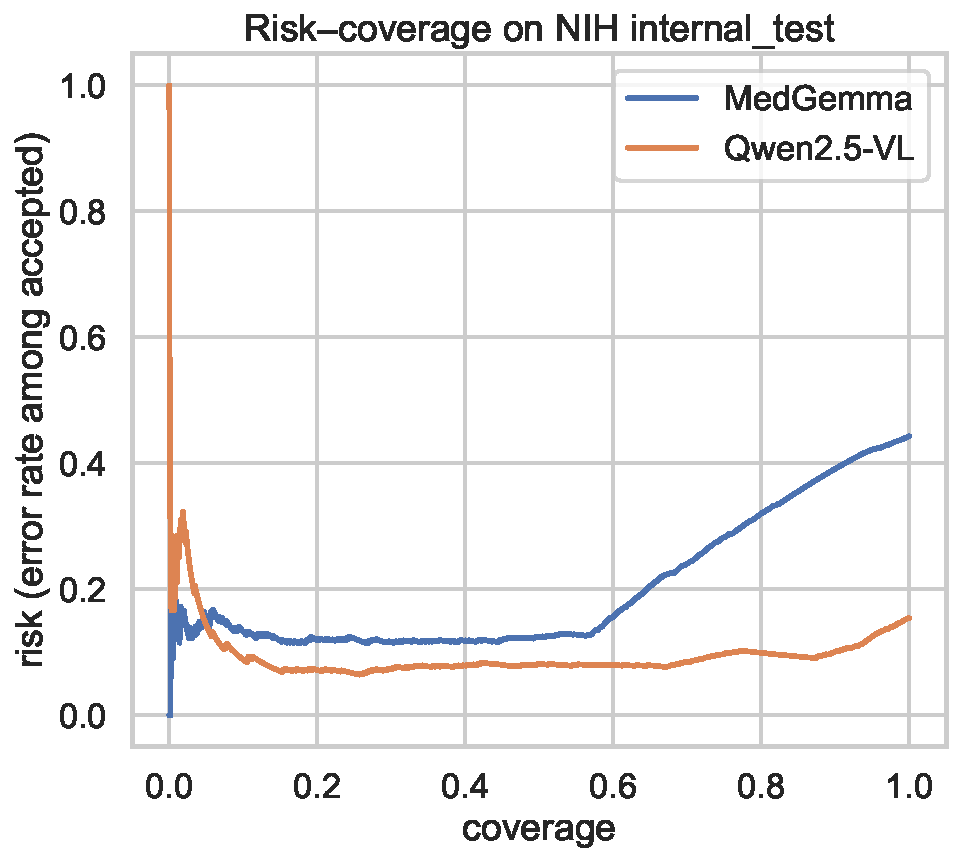
\includegraphics[width=0.75\linewidth]{figures/fig06_risk_coverage.pdf}
  \caption{Risk--coverage curves on NIH internal test data. Qwen2.5-VL appears favourable despite image-invariant predictions, highlighting that selective risk must be conditioned on image reliance.}
  \label{fig:risk-coverage}
\end{figure}

\begin{figure}[t]
  \centering
  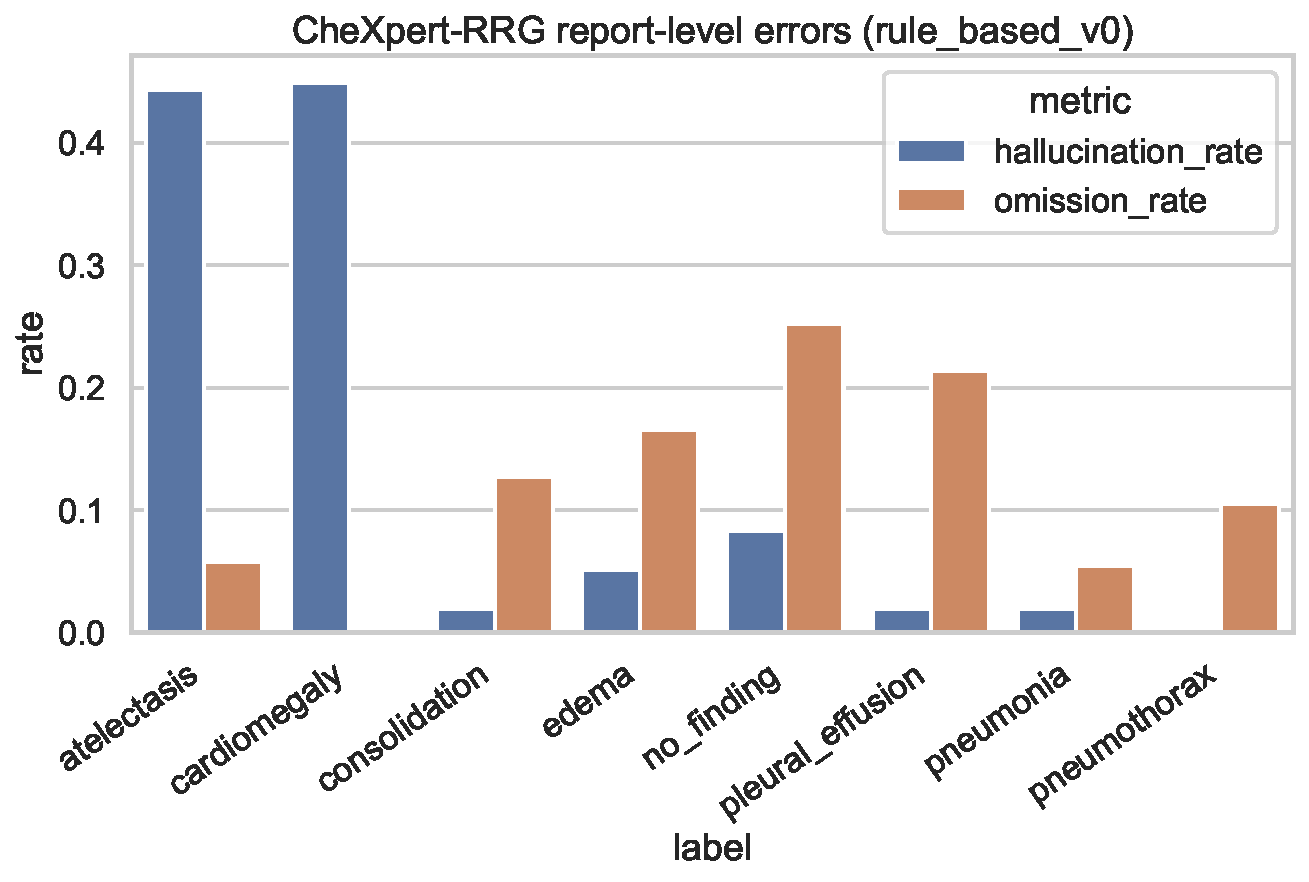
\includegraphics[width=\linewidth]{figures/fig07_rrg_report_errors.pdf}
  \caption{Finding-level hallucination and omission on CheXpert-plus-RRG using the pilot rule-based evidence extractor. These results require validation with a dedicated report labeller.}
  \label{fig:rrg-errors}
\end{figure}

\begin{figure}[t]
  \centering
  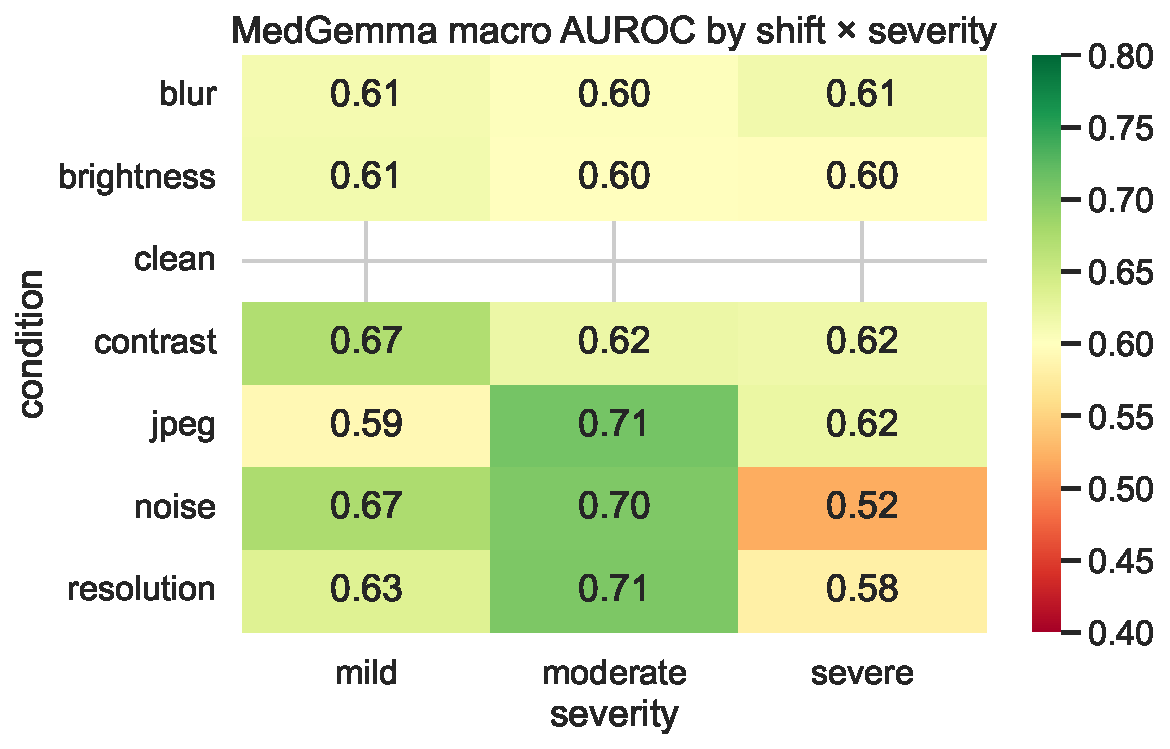
\includegraphics[width=0.75\linewidth]{figures/fig08_shift_macro_auroc_heatmap.pdf}
  \caption{MedGemma macro AUROC across shift conditions and severity levels.}
  \label{fig:shift-heatmap}
\end{figure}

\begin{figure}[t]
  \centering
  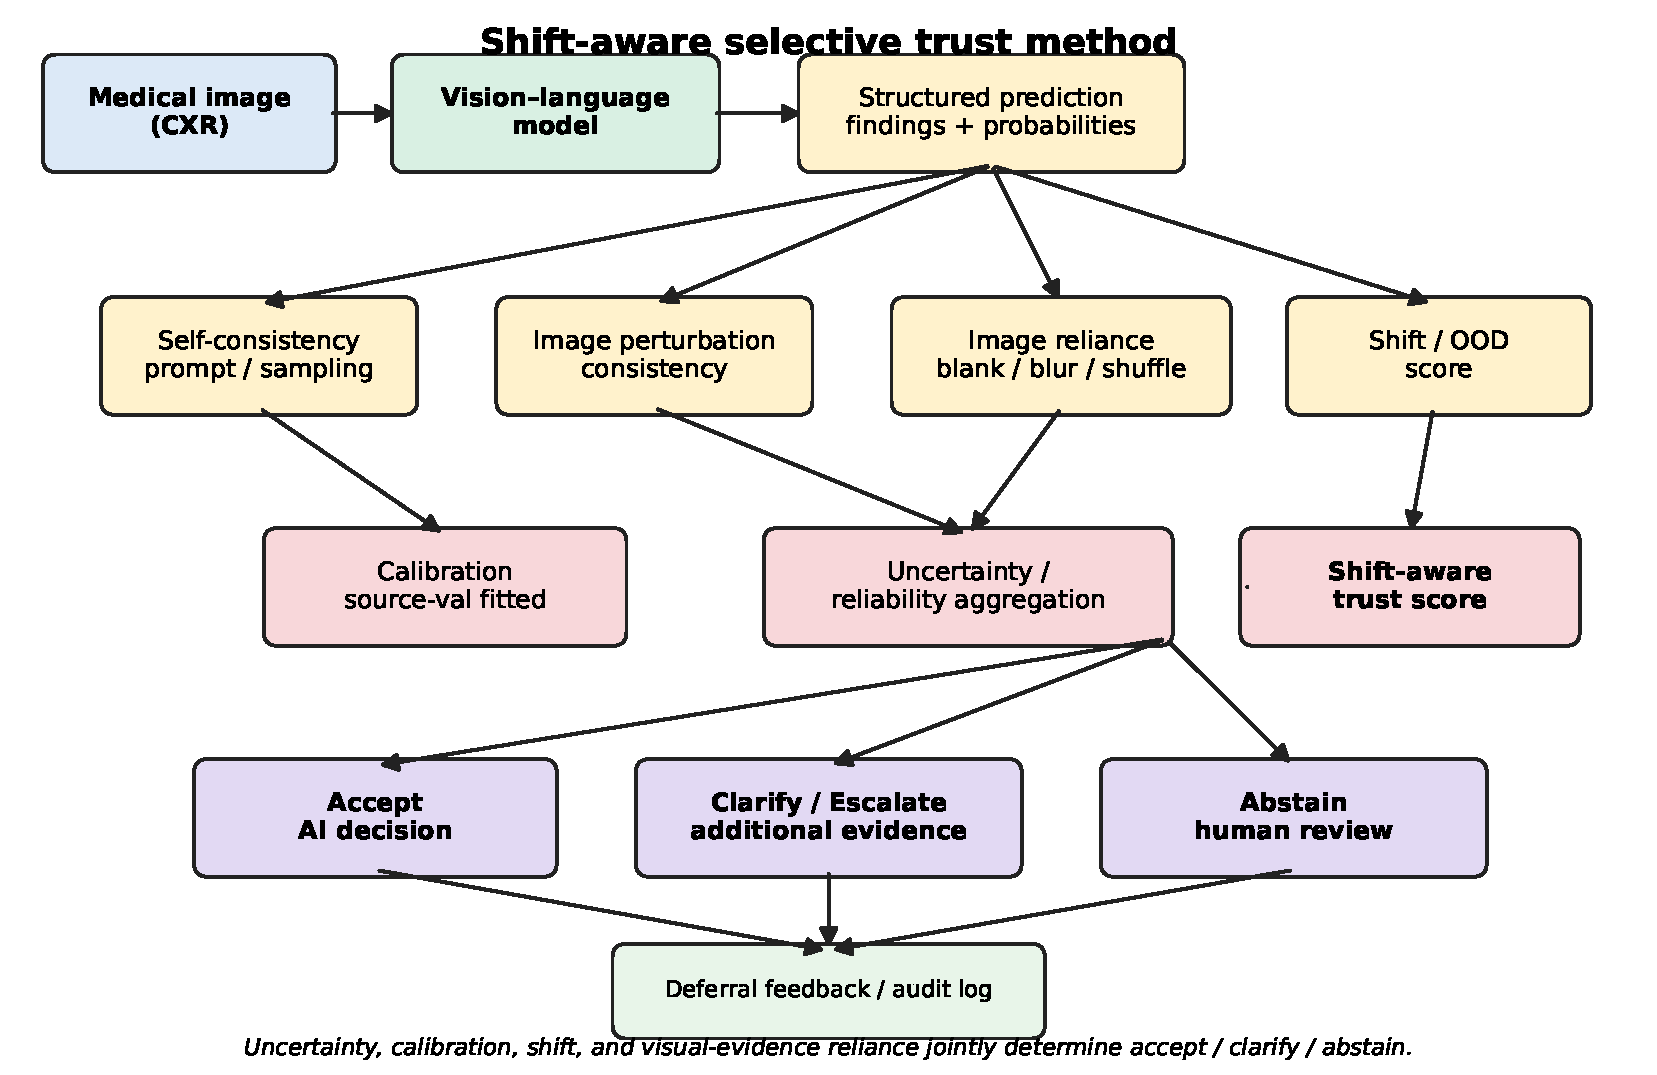
\includegraphics[width=\linewidth]{figures/fig09_selective_trust_method.pdf}
  \caption{Detailed selective trust method, including uncertainty, calibration, image reliance, and shift-aware aggregation.}
  \label{fig:method}
\end{figure}

\begin{figure}[t]
  \centering
  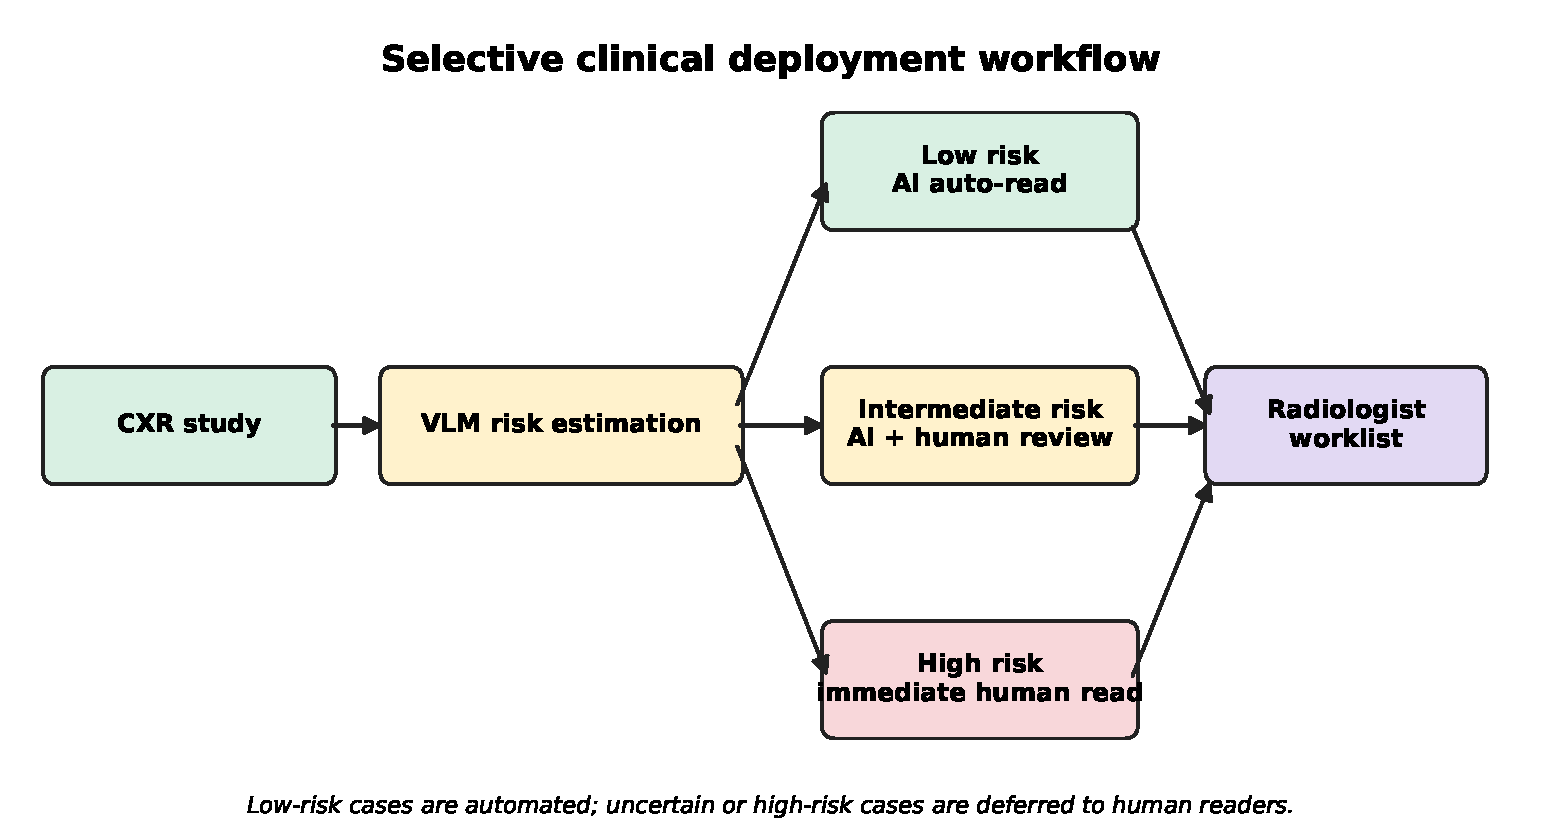
\includegraphics[width=\linewidth]{figures/fig10_clinical_workflow.pdf}
  \caption{Clinical selective deployment workflow. Low-risk cases are automated, intermediate-risk cases are reviewed with AI assistance, and high-risk cases are deferred to immediate human review.}
  \label{fig:workflow}
\end{figure}
